
%(BEGIN_QUESTION)
% Copyright 2006, Tony R. Kuphaldt, released under the Creative Commons Attribution License (v 1.0)
% This means you may do almost anything with this work of mine, so long as you give me proper credit

Suppose that a liquid is placed into a container, and then all the air is drawn out of that container using a vacuum pump:

$$\includegraphics[width=15.5cm]{i00348x01.eps}$$

The container is then sealed, and the absolute pressure measured with some kind of pressure instrument:

$$\includegraphics[width=15.5cm]{i00348x02.eps}$$

As the liquid is trapped inside the container, thermal energy liberates some of the molecules into the vacuum above, resulting in a vapor forming above the liquid.  As some of these vapor molecules strike the walls of the container, they condense back into liquid and dribble down into the liquid pool below.  When the rates of evaporation and condensation reach equilibrium, we say the liquid/vapor process is in a condition of {\it saturation}, and the amount of pressure inside this vessel as the {\it saturated vapor pressure} of the substance.  ``Saturated'' simply refers to the condition where the rates of evaporation and condensation exactly match; when the space above the liquid can hold no more vapor molecules.

\vskip 10pt

Suppose we now attach a piston to this container so we may change the volume of the vapor space:

$$\includegraphics[width=15.5cm]{i00348x03.eps}$$

If the system reaches a state of saturation (evaporation and condensation rates equal), and temperature remains the same, what will happen to the pressure in the container if the piston is moved inward, thus decreasing volume?  Does the pressure increase, decrease, or stay the same?

\vskip 10pt

Now suppose we attach a pump to the bottom of this container so we may remove some of the liquid without letting any air in:

$$\includegraphics[width=15.5cm]{i00348x04.eps}$$

If the system reaches a state of saturation (evaporation and condensation rates equal), and temperature remains the same, what will happen to the pressure in the container as liquid is drawn out?  Does the pressure increase, decrease, or stay the same?

\underbar{file i00348}
%(END_QUESTION)





%(BEGIN_ANSWER)

In both cases (piston moving in, and pump pulling liquid out) there will be an initial change in pressure.  However, the pressure will stabilize at the exact same quantity it was at before once equilibrium is re-established.  Saturated vapor pressure does not depend on the quantity of liquid or vapor, or the volume of the enclosed space!

Initially, the pressure will increase because the vapor will be forced into a smaller volume (remember $PV = nRT$).  This will cause the rate of condensation (vapor-to-liquid) to increase and the rate of evaporation (liquid-to-vapor) to decrease.  As excess vapor re-condenses into liquid, the pressure will decrease due to a lesser molar quantity of vapor (the $n$ in $PV = nRT$) in the space above the liquid.  Eventually, the pressure will stabilize at the exact same quantity it was at before, when the system reaches a state of saturation again.  

%(END_ANSWER)





%(BEGIN_NOTES)

%INDEX% Physics, heat and temperature: saturated vapor pressure

%(END_NOTES)


